\begin{frame}[fragile]{Visualização da chamada $F(5)$}

    \begin{figure}
        \centering

        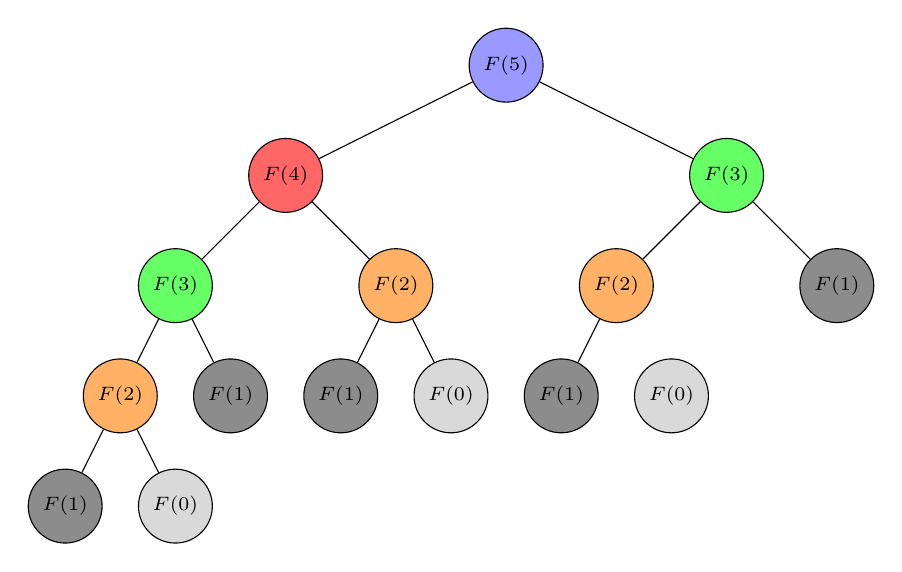
\begin{tikzpicture}[scale=0.7]
            \node[draw,circle,fill=blue!40] (A) at (6, 6) { \scriptsize $F(5)$ };
            \node[draw,circle,fill=red!60] (B) at (2, 4) { \scriptsize $F(4)$ };
            \node[draw,circle,fill=green!60] (C) at (10, 4) { \scriptsize $F(3)$ };
            \node[draw,circle,fill=green!60] (D) at (0, 2) { \scriptsize $F(3)$ };
            \node[draw,circle,fill=orange!60] (E) at (4, 2) { \scriptsize $F(2)$ };
            \node[draw,circle,fill=orange!60] (F) at (8, 2) { \scriptsize $F(2)$ };
            \node[draw,circle,fill=gray!90] (G) at (12, 2) { \scriptsize $F(1)$ };
            \node[draw,circle,fill=orange!60] (H) at (-1, 0) { \scriptsize $F(2)$ };
            \node[draw,circle,fill=gray!90] (I) at (1, 0) { \scriptsize $F(1)$ };
            \node[draw,circle,fill=gray!90] (J) at (3, 0) { \scriptsize $F(1)$ };
            \node[draw,circle,fill=gray!30] (K) at (5, 0) { \scriptsize $F(0)$ };
            \node[draw,circle,fill=gray!90] (L) at (7, 0) { \scriptsize $F(1)$ };
            \node[draw,circle,fill=gray!30] (M) at (9, 0) { \scriptsize $F(0)$ };
            \node[draw,circle,fill=gray!90] (N) at (-2, -2) { \scriptsize $F(1)$ };
            \node[draw,circle,fill=gray!30] (O) at (0, -2) { \scriptsize $F(0)$ };

            \draw (A) edge (B);
            \draw (A) edge (C);
            \draw (B) edge (D);
            \draw (B) edge (E);
            \draw (C) edge (F);
            \draw (C) edge (G);
            \draw (D) edge (H);
            \draw (D) edge (I);
            \draw (E) edge (J);
            \draw (E) edge (K);
            \draw (F) edge (L);
            \draw (H) edge (N);
            \draw (H) edge (O);

        \end{tikzpicture}

    \end{figure}

\end{frame}
